%implementing document formatting:
\documentclass[a4paper,11pt,fleqn,dvipsnames,oneside,openright,oldfontcommands]{memoir} 	% Openright aabner kapitler paa hoejresider (openany begge)


%%%%%%%%% Indsat random
%makes it possible to refer to the name of a chapter rather than just the number.
\usepackage{nameref}





% ¤¤ Litteraturlisten ¤¤ %
%setting references (using numbers) and supporting i.a. Chicargo-style:
\usepackage{etex}
\usepackage{etoolbox}
\usepackage{keyval}
\usepackage{ifthen}
\usepackage{url}
\usepackage{csquotes}
\usepackage[numbers]{natbib}
%\newcommand{\btx}{Bib\TeX}
%\usepackage[backend=biber,url=true,doi=true,style=numeric, sorting=none]{biblatex}
%\addbibresource{VoresKilder.bib}















%package for writing program code in latex
\usepackage{listings}
%%%%%%%%%%%%%%%%%%%%%%

% ¤¤ Oversaettelse og tegnsaetning ¤¤ %
\usepackage[utf8]{inputenc}					% Input-indkodning af tegnsaet (UTF8)
\usepackage[danish]{babel}					% Dokumentets sprog
\usepackage[T1]{fontenc}					% Output-indkodning af tegnsaet (T1)
\usepackage{ragged2e,anyfontsize}			% Justering af elementer
\usepackage{fixltx2e}						% Retter forskellige fejl i LaTeX-kernen							
								
								
								
																			
% ¤¤ Figurer og tabeller (floats) ¤¤ %
\usepackage{graphicx} 						% Haandtering af eksterne billeder (JPG, PNG, EPS, PDF)
%\usepackage{eso-pic}						% Tilfoej billedekommandoer paa hver side
%\usepackage{wrapfig}						% Indsaettelse af figurer omsvoebt af tekst. \begin{wrapfigure}{Placering}{Stoerrelse}
\usepackage{multirow}                		% Fletning af raekker og kolonner (\multicolumn og \multirow)
\usepackage{multicol}         	        	% Muliggoer output i spalter
\usepackage{rotating}						% Rotation af tekst med \begin{sideways}...\end{sideways}
\usepackage{colortbl} 						% Farver i tabeller (fx \columncolor og \rowcolor)
\usepackage{xcolor}							% Definer farver med \definecolor. Se mere: http://en.wikibooks.org/wiki/LaTeX/Colors
\usepackage{flafter}						% Soerger for at floats ikke optraeder i teksten foer deres reference
\let\newfloat\relax 						% Justering mellem float-pakken og memoir
\usepackage{float}							% Muliggoer eksakt placering af floats, f.eks. \begin{figure}[H]
\usepackage{array,booktabs,xcolor,longtable} % kan lave \hdashline i tabellertabe
\usepackage{arydshln}
\usepackage{tabu}

	
	
% ¤¤ Matematik mm. ¤¤
\usepackage{amsmath , amsfonts , amssymb, float, stmaryrd} 		% Avancerede matematik-udvidelser
%\usepackage{mathtools}						% Andre matematik- og tegnudvidelser
\usepackage{textcomp}                 		% Symbol-udvidelser (f.eks. promille-tegn med \textperthousand )
\usepackage{rsphrase}						% Kemi-pakke til RS-saetninger, f.eks. \rsphrase{R1}
\usepackage[version=3]{mhchem} 				% Kemi-pakke til flot og let notation af formler, f.eks. \ce{Fe2O3}
\usepackage{siunitx}						% Flot og konsistent praesentation af tal og enheder med \si{enhed} og \SI{tal}{enhed}
\sisetup{output-decimal-marker = {,}}		% Opsaetning af \SI (DE for komma som decimalseparator) 

% ¤¤ Referencer og kilder ¤¤ %
\usepackage[danish]{varioref}				% Muliggoer bl.a. krydshenvisninger med sidetal (\vref)
\usepackage[numbers]{natbib}				% Udvidelse med naturvidenskabelige citationsmodeller
%\usepackage{xr}							% Referencer til eksternt dokument med \externaldocument{<NAVN>}
%\usepackage{glossaries}					% Terminologi- eller symbolliste (se mere i Daleifs Latex-bog)
\usepackage{lastpage}					% Gør det mulig at refere til sidste side 

% ¤¤ Misc. ¤¤ %
\usepackage{listings}						% Placer kildekode i dokumentet med \begin{lstlisting}...\end{lstlisting}
\usepackage{lipsum}							% Dummy text \lipsum[..]
\usepackage[shortlabels]{enumitem}			% Muliggoer enkelt konfiguration af lister
\usepackage{pdfpages}						% Goer det muligt at inkludere pdf-dokumenter med kommandoen \includepdf[pages={x-y}]{fil.pdf}	
\pdfoptionpdfminorversion=6					% Muliggoer inkludering af pdf dokumenter, af version 1.6 og hoejere
\pretolerance=2500 							% Justering af afstand mellem ord (hoejt tal, mindre orddeling og mere luft mellem ord)


% Kommentarer og rettelser med \fxnote. Med 'final' i stedet for 'draft' udloeser hver note en error i den faerdige rapport.
\usepackage[footnote,draft,danish,silent,nomargin]{fixme}		


%%%% CUSTOM SETTINGS %%%%

% ¤¤ Marginer ¤¤ %
\setlrmarginsandblock{3.5cm}{2.5cm}{*}		% \setlrmarginsandblock{Indbinding}{Kant}{Ratio}
\setulmarginsandblock{2.5cm}{3.0cm}{*}		% \setulmarginsandblock{Top}{Bund}{Ratio}
\checkandfixthelayout 						% Oversaetter vaerdier til brug for andre pakker

%	¤¤ Afsnitsformatering ¤¤ %
\setlength{\parindent}{6mm}           		% Stoerrelse af indryk
\setlength{\parskip}{0mm}          			% Afstand mellem afsnit ved brug af double Enter
\linespread{1,1}							% Linie afstand



% ¤¤ Indholdsfortegnelse ¤¤ %
\setsecnumdepth{subsection}		 			% Dybden af nummerede overkrifter (part/chapter/section/subsection)
\maxsecnumdepth{subsection}					% Dokumentklassens graense for nummereringsdybde
\settocdepth{subsection} 					% Dybden af indholdsfortegnelsen

% ¤¤ Lister ¤¤ %
\setlist{
  topsep=0pt,								% Vertikal afstand mellem tekst og listen
  itemsep=-1ex,								% Vertikal afstand mellem items
} 

%hyperlinks in the tabel of contents - comment this out before the report is printed.
\usepackage{hyperref}
\hypersetup{
	bookmarks = true,  % Show 'bookmark'-frame in pdf.
	colorlinks = true, % True = colored links, False = framed links.
	citecolor = black,  % Link color for references.
	linkcolor = black,  % Link color in table of contents.
	urlcolor = black,   % Link color for extern URLs.
}

% ¤¤ Opsaetning af figur- og tabeltekst ¤¤ %
\usepackage{caption}
\usepackage{subcaption}
\captionnamefont{\small\bfseries\itshape}	% Opsaetning af tekstdelen ('Figur' eller 'Tabel')
\captiontitlefont{\small}					% Opsaetning af nummerering
\captiondelim{. }							% Seperator mellem nummerering og figurtekst
\hangcaption								% Venstrejusterer flere-liniers figurtekst under hinanden
%\captionwidth{0.9\textwidth}					% Bredden af figurteksten
\setlength{\belowcaptionskip}{0pt}			% Afstand under figurteksten
\captionsetup[figure]{labelfont={bf,it},font={it}} % sætter nummer til fed og kursis. Resten til fed + skriften er mindre end resten
\captionsetup[table]{labelfont={bf,it},font={it}} 


% ¤¤ Opsaetning af listings ¤¤ %

\definecolor{commentGreen}{RGB}{34,139,24}
\definecolor{stringPurple}{RGB}{208,76,239}

\lstset{language=Matlab,					% Sprog
	basicstyle=\ttfamily\scriptsize,		% Opsaetning af teksten
	keywords={for,if,while,else,elseif,		% Noegleord at fremhaeve
			  end,break,return,case,
			  switch,function},
	keywordstyle=\color{blue},				% Opsaetning af noegleord
	commentstyle=\color{commentGreen},		% Opsaetning af kommentarer
	stringstyle=\color{stringPurple},		% Opsaetning af strenge
	showstringspaces=false,					% Mellemrum i strenge enten vist eller blanke
	numbers=left, numberstyle=\tiny,		% Linjenumre
	extendedchars=true, 					% Tillader specielle karakterer
	columns=flexible,						% Kolonnejustering
	breaklines, breakatwhitespace=true,		% Bryd lange linjer
}

% ¤¤ Navngivning ¤¤ %
\addto\captionsdanish{
	\renewcommand\appendixname{Bilag}
	\renewcommand\contentsname{Indholdsfortegnelse}	
	\renewcommand\appendixpagename{Bilag}
	\renewcommand\appendixtocname{Bilag}
	\renewcommand\cftchaptername{\chaptername~}				% Skriver "Kapitel" foran kapitlerne i indholdsfortegnelsen
	\renewcommand\cftappendixname{\appendixname~}			% Skriver "Appendiks" foran appendiks i indholdsfortegnelsen
}

% ¤¤ Kapiteludssende ¤¤ %
%\definecolor{numbercolor}{gray}{0.7}		% Definerer en farve til brug til kapiteludseende
%\newif\ifchapternonum

\makechapterstyle{AAU}
{
	% Afstand mellem sidehovedet og kapitel+tal+kapitelnavnet defineres til:
	\setlength{\beforechapskip}{0cm}

	% Afstanden mellem kapitelnavnet og body-teksten defineres til:
	\setlength{\afterchapskip}{2cm}

	% Typografiopsætningen til kapitel+tal defineres til:
	\renewcommand\chapnamefont{\sffamily\bfseries\LARGE\raggedright}
	
	% Typografiopsætningen til kapitel+tal defineres til:
	\renewcommand\chaptitlefont{\sffamily\bfseries\huge\color[cmyk]{1.00,0.38,0.00,0.64}}

	% Forårsager, at der til kapitlet også tilføjes dets respektive tal:
	\renewcommand\chapternamenum{}
	\renewcommand\printchapternum
	{
		\makebox[0pt][l]
		{
			\color[cmyk]{1.00,0.38,0.00,0.64}
			\hspace{0.1cm}
			\resizebox{!}{1cm}{\chapnamefont\bfseries\sffamily\thechapter}
		}
	}
	
	% Definitionen af linjenstykket mellem ``Kapitel #'' samt ``kapitelnavnet'':
			\renewcommand\afterchaptertitle{\par\hspace{1.5cm}\hrule height 1pt\vskip\midchapskip}
}

% Aktivering af selve kapitellayoutet med dét navn, som definerer kapitellayoutet (ses fra tidligere):
\chapterstyle{AAU}

%\makechapterstyle{jenor}{					% Definerer kapiteludseende frem til ...
%  \renewcommand\beforechapskip{0pt}
%  \renewcommand\printchaptername{}
%  \renewcommand\printchapternum{}
% % \renewcommand\printchapternonum{\chapternonumtrue}
%  \renewcommand\chaptitlefont{\fontfamily{pbk}\fontseries{db}\fontshape{n}\fontsize{20}{25}\selectfont\raggedright}
%  \renewcommand\chapnumfont{\fontfamily{pbk}\fontseries{m}\fontshape{n}\fontsize{1in}{0in}\selectfont\color{numbercolor}}
% \renewcommand\printchaptertitle[1]{
%    \noindent
%    \ifchapternum
%     \begin{tabularx}{\textwidth}{XI}
%	{\let\\\newline\chaptitlefont ##1\par}     
%    \end{tabularx}
%    \par\vskip-2.5mm\hrule
%    \else
%    \begin{tabularx}{\textwidth}{X}
%      {\parbox[b]{\linewidth}{\chaptitlefont ##1}} & \raisebox{-15pt}{\chapnumfont \thechapter}
%    \end{tabularx}
%    \par\vskip2mm\hrule
%    \fi
%  }
%}											% ... her
%
%\chapterstyle{jenor}						% Valg af kapiteludseende - Google 'memoir chapter styles' for alternativer

% ¤¤ Sidehoved ¤¤ %

\makepagestyle{AAU}							% Definerer sidehoved og sidefod udseende frem til ...
\makepsmarks{AAU}{%
	\createmark{chapter}{left}{shownumber}{}{. \ }
	\createmark{section}{right}{shownumber}{}{. \ }
	\createplainmark{toc}{both}{\contentsname}
	\createplainmark{lof}{both}{\listfigurename}
	\createplainmark{lot}{both}{\listtablename}
	%\createplainmark{bib}{both}{\bibname}
	\createplainmark{index}{both}{\indexname}
	\createplainmark{glossary}{both}{\glossaryname}
}
\nouppercaseheads											% Ingen Caps oenskes

\makeoddhead{AAU}{Gruppe B206}{}{\leftmark}				% Definerer lige siders sidehoved (\makeevenhead{Navn}{Venstre}{Center}{Hoejre})
\makeevenhead{AAU}{\rightmark}{}{Aalborg Universitet}		% Definerer ulige siders sidehoved (\makeoddhead{Navn}{Venstre}{Center}{Hoejre})
\makeevenfoot{AAU}{\thepage\ af \pageref{LastPage}}{}{}							% Definerer lige siders sidefod (\makeevenfoot{Navn}{Venstre}{Center}{Hoejre})
\makeoddfoot{AAU}{}{}{\thepage\ af \pageref{LastPage}}								% Definerer ulige siders sidefod (\makeoddfoot{Navn}{Venstre}{Center}{Hoejre})
\makeheadrule{AAU}{\textwidth}{0.5pt}						% Tilfoejer en streg under sidehovedets indhold
\makefootrule{AAU}{\textwidth}{0.5pt}{1mm}					% Tilfoejer en streg under sidefodens indhold

\copypagestyle{AAUchap}{AAU}								% Sidehoved for kapitelsider defineres som standardsider, men med blank sidehoved
\makeoddhead{AAUchap}{}{}{}
\makeevenhead{AAUchap}{}{}{}
\makeheadrule{AAUchap}{\textwidth}{0pt}
\aliaspagestyle{chapter}{AAUchap}							% Den ny style vaelges til at gaelde for chapters
															% ... her
															
\pagestyle{AAU}												% Valg af sidehoved og sidefod


%%%% CUSTOM COMMANDS %%%%

% ¤¤ Billede hack ¤¤ %
\newcommand{\figur}[4]{
		\begin{figure}[H] \centering
			\includegraphics[width=#1\textwidth]{billeder/#2}
			\caption{#3}\label{#4}
		\end{figure} 
}

% ¤¤ Specielle tegn ¤¤ %
\newcommand{\decC}{^{\circ}\text{C}}
\newcommand{\dec}{^{\circ}}
\newcommand{\m}{\cdot}


%%%% ORDDELING %%%%

\hyphenation{}

%%%%Fra engelsk til dansk i \autoref{•} %%%%
\renewcommand{\figureautorefname}{Figur}
\renewcommand{\sectionautorefname}{Afsnit}
\renewcommand{\subsectionautorefname}{Afsnit}
\renewcommand{\subsubsectionautorefname}{Afsnit}
\renewcommand{\tableautorefname}{Tabel}
\renewcommand{\appendixautorefname}{Bilag}
\renewcommand{\equationautorefname}{Ligning}
\renewcommand{\itemautorefname}{Punkt}
\renewcommand{\chapterautorefname}{Kapitel}
\usepackage{marvosym}
%Figure references:
\newcommand{\figref}[1]{\textbf{figure \ref{#1}}}

%Figure references after full stop/period:
\newcommand{\Figref}[1]{\textbf{Figure \ref{#1}}}

%Table references:
\newcommand{\tableref}[1]{\textbf{table \ref{#1}}}

%Table references after full stop/period:
\newcommand{\Tableref}[1]{\textbf{Table \ref{#1}}}

%Units:
%inserting '\omit' before '{\put' prior ot final compile will fix allignment (and generate errors)
\newcommand{\unit}[1]{{\put(300,0){$\hfill\left[\: #1 \:\right]$}}}

%Text:
\newcommand{\tx}[1]{\text{#1}}

%Equation references:
%1 equation:
\renewcommand{\eqref}[1]{\textbf{equation (\ref{#1})}}
%2 equations:
\newcommand{\eqrefTwo}[2]{\textbf{equation (\ref{#1})} and \textbf{(\ref{#2})}}
%3 equations:
\newcommand{\eqrefThree}[3]{\textbf{equation (\ref{#1})}, \textbf{(\ref{#2})} and \textbf{(\ref{#3})}}
%4 equations:
\newcommand{\eqrefFour}[4]{\textbf{equation (\ref{#1})}, \textbf{(\ref{#2})}, \textbf{(\ref{#3})} and \textbf{(\ref{#4})}}
%5 equations:
\newcommand{\eqrefFive}[5]{\textbf{equation (\ref{#1})}, \textbf{(\ref{#2})}, \textbf{(\ref{#3})}, \textbf{(\ref{#4})} and \textbf{(\ref{#5})}}
%5 equations:
\newcommand{\eqrefSix}[6]{\textbf{equation (\ref{#1})}, \textbf{(\ref{#2})}, \textbf{(\ref{#3})}, \textbf{(\ref{#4})}, \textbf{(\ref{#5})} and \textbf{(\ref{#6})}}
%5 equations:
\newcommand{\eqrefSeven}[7]{\textbf{equation (\ref{#1})}, \textbf{(\ref{#2})}, \textbf{(\ref{#3})}, \textbf{(\ref{#4})}, \textbf{(\ref{#5})}, \textbf{(\ref{#6})} and \textbf{(\ref{#7})}}

%Equation references after full stop/period:
%1 equation:
\newcommand{\Eqref}[1]{\textbf{Equation (\ref{#1})}}
%2 equations:
\newcommand{\EqrefTwo}[2]{\textbf{Equation (\ref{#1})} and \textbf{(\ref{#2})}}
%3 equations:
\newcommand{\EqrefThree}[3]{\textbf{Equation (\ref{#1})}, \textbf{(\ref{#2})} and \textbf{(\ref{#3})}}
%4 equations:
\newcommand{\EqrefFour}[4]{\textbf{Equation (\ref{#1})}, \textbf{(\ref{#2})}, \textbf{(\ref{#3})} and \textbf{(\ref{#4})}}
%5 equations:
\newcommand{\EqrefFive}[5]{\textbf{Equation (\ref{#1})}, \textbf{(\ref{#2})}, \textbf{(\ref{#3})}, \textbf{(\ref{#4})} and \textbf{(\ref{#5})}}
%5 equations:
\newcommand{\EqrefSix}[6]{\textbf{Equation (\ref{#1})}, \textbf{(\ref{#2})}, \textbf{(\ref{#3})}, \textbf{(\ref{#4})}, \textbf{(\ref{#5})} and \textbf{(\ref{#6})}}
%5 equations:
\newcommand{\EqrefSeven}[7]{\textbf{Equation (\ref{#1})}, \textbf{(\ref{#2})}, \textbf{(\ref{#3})}, \textbf{(\ref{#4})}, \textbf{(\ref{#5})}, \textbf{(\ref{#6})} and \textbf{(\ref{#7})}}
\begin{document}

%||||||||||||||||||||||||||||||||||||||||||||||||||||||||||||||||
%|||||||				Example Inputs					 ||||||||
%||||||||||||||||||||||||||||||||||||||||||||||||||||||||||||||||
%|||||||												 ||||||||
%	\section{Figure Sample}

\begin{figure}[H]
	\caption{CAPTION\fxnote{Remember source}}
	\label{LABEL}
	\centering
	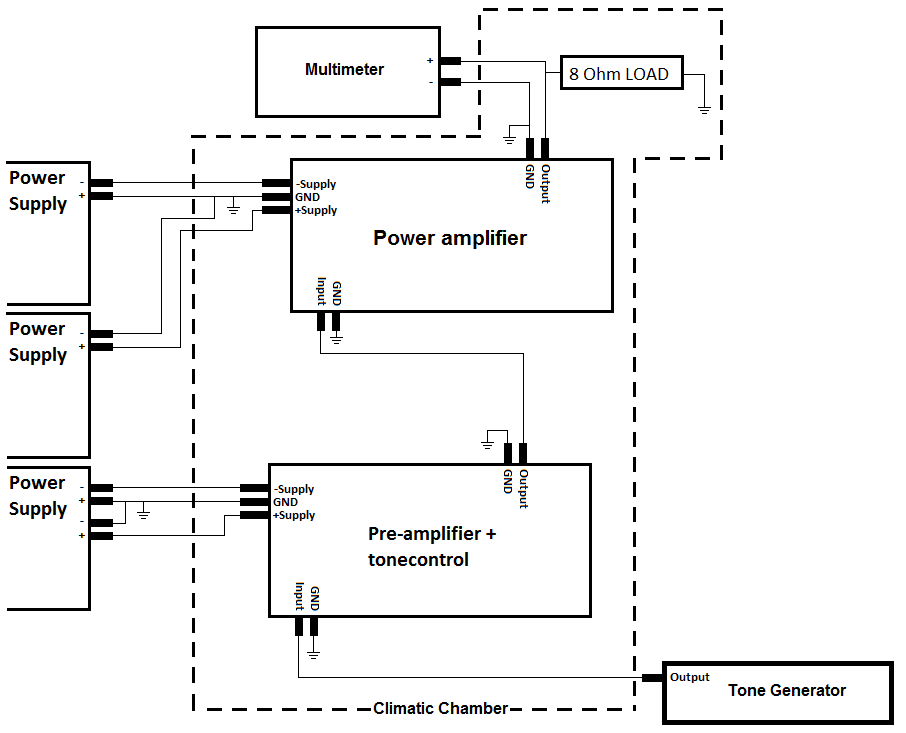
\includegraphics[scale=.8]{figures/filename}
	\flushleft
	\textit{SOURCE}
\end{figure}

%--------- NOTES ------------------------------------------------------
%Fxnotes wont compile properly inside the figure, only in the caption.
%Filetype can be specified but isn't needed.

\noindent
\figref{LABEL}\\

\noindent
\Figref{LABEL}

\vspace{.5cm}
%Do not use \vspace{length} or \hspace{length} unless exceedingly necessary.

%--------- BIBLIOGRAPHY REF EKSAMPLE -----------------------------------
This reference only represents this line since it is before the punctuation mark\cite{YDing}. This next reference however represents the entire section. That is all of the preceding sentences in the entire section. This is due to the fact that it is now after the punctuation mark in the end of the section (this is not used in the middle of a section!).\cite{YDing}
%>>>>>>>>>>>>>>>PLEASE ALSO READ THE NOTE IN myBib.bib<<<<<<<<<<<<<<<<<<
\pagebreak	%||||||||
%	\section{Table Sample}

\begin{table}[H]
\caption{This Is a Table\label{LABEL}}
\begin{tabular}{|l|p{5cm}|l|l|l|}
  \hline
  \textbf{No.}&\textbf{Description}&\textbf{Min}&\textbf{Max}&\textbf{Requirements}\\
  \hline
  1 & Some Text & Some Text & Some Text & Some Text\\
    &           &           &           & Some More Text\\
    &           &           &           & Text Text\\
    &           &           &           & Text Text Text\\
  \hline
  2 & Some Text & Some Text & Some Text & Some Text\\
  \hline
  3 & 	By specifying the width of a column (|p\{5cm\}|) the cells
  		in that column will will not exceed	the specified width    %Enter is used only for clarity and will not affect the compiled output.
  		but instead expand downward.
  		
  		        & Some Text & Some Text & Some Text\\
  \hline
  4 & Some Text & Some Text & Some Text & Some Text\\
  \hline
  \multicolumn{2}{|l|}{Some Text} 	&	\multicolumn{3}{l|}{Some Text}\\
  \hline
  \multicolumn{2}{|l|}{Text Text} 	&	\multicolumn{3}{l|}{Text = Text}\\
  \multicolumn{2}{|l|}{}			&	\multicolumn{3}{l|}{Text = Text}\\
  \multicolumn{2}{|l|}{}			&	\multicolumn{3}{l|}{Text = Text}\\
  \multicolumn{2}{|l|}{}			&	\multicolumn{3}{l|}{Text = Text}\\
  \multicolumn{2}{|l|}{}			&	\multicolumn{3}{l|}{Text = Text}\\
  \hline
  \multicolumn{2}{|l|}{Some Text} 	&	\multicolumn{3}{l|}{Teeeexxtt}\\
  \multicolumn{2}{|l|}{}			&	\multicolumn{3}{l|}{\LaTeX}\\
  \hline      
\end{tabular}
\end{table}

\noindent
\tableref{LABEL}\\

\noindent
\Tableref{LABEL}

\pagebreak	%||||||||
%	\section{Equation Sample}

\noindent
Some explanation:
%
\begin{align}
\unit{Unit}
[Equation]&=[Number]
\label{eq1}
\end{align}

\noindent
Some other explanation:
%
\begin{align}
\unit{Unit}
[Equation]&=[Number]
\label{eq2}
\end{align}

\noindent
Yet an explanation:
%
\begin{align}
\unit{Unit}
\text{You see? } [Equation]&=[Number]
\label{eq3}\\
%
\unit{Unit}
\text{Unit isn't aligned } \textbf{:( } \: [Equation]&=[Number]
\label{eq4}	   %
\end{align}	 	%
			  	 %
\noindent	   	  %
Explanation!:	   %
%				 	%
\begin{align}	  	 %
\unit{Unit}		   	  %
[Equation]&=[Number]   %	%-----------------------NOTES-----------------------%
\label{eq5}\\		 	%	% The &-sign aligns the equal signs.				%
%					  	 %	%													%
\unit{Unit}			   	  % % \unit{} will not be alligned by default,			%
[Equation]&=[Number]	   %% however the macro can be modded as described 		%
\label{eq6}\\			    % in macros.tex. This will allign the units,		%
%						    % but generate errors.								%
\unit{Unit}				    %													%
[Equation]&=[Number]		% \noindent should generally be used befor			%
\label{eq7}					% oneliners after equations, figures and tables.	%
\end{align}					%---------------------------------------------------%
\\
%
\noindent
\eqref{eq1}\\
\noindent
\eqrefTwo{eq1}{eq2}\\
\noindent
\eqrefThree{eq1}{eq2}{eq3}\\
\noindent
\eqrefFour{eq1}{eq2}{eq3}{eq4}\\
\noindent
\eqrefFive{eq1}{eq2}{eq3}{eq4}{eq5}\\
\noindent
\eqrefSix{eq1}{eq2}{eq3}{eq4}{eq5}{eq6}\\
\noindent
\eqrefSeven{eq1}{eq2}{eq3}{eq4}{eq5}{eq6}{eq7}\\
\noindent
\Eqref{eq1}\\
\noindent
\EqrefTwo{eq1}{eq2}\\
\noindent
\EqrefThree{eq1}{eq2}{eq3}\\
\noindent
\EqrefFour{eq1}{eq2}{eq3}{eq4}\\
\noindent
\EqrefFive{eq1}{eq2}{eq3}{eq4}{eq5}\\
\noindent
\EqrefSix{eq1}{eq2}{eq3}{eq4}{eq5}{eq6}\\
\noindent
\EqrefSeven{eq1}{eq2}{eq3}{eq4}{eq5}{eq6}{eq7}
\pagebreak	%||||||||
%|||||||												 ||||||||
%||||||||||||||||||||||||||||||||||||||||||||||||||||||||||||||||
%||||||||||||||||||||||||||||||||||||||||||||||||||||||||||||||||


%---------------------------INPUTS-------------------------------
%numbers the pages with Roman numeral - starts from "i":
\frontmatter

\clearpage
\thispagestyle{empty}

%\begin{figure}[H]
%	\raggedleft
%		
\includegraphics[width=0.2\textwidth]{figures/aaulogo-da.png}
%\end{figure}


%\vspace*{\fill} 
%\begin{center}	
%	\begin{Huge}
%		P3 Projektrapport - efterår 2015\\
%		\vspace{5 mm}
%		\textbf{System til detektering af kropsbalance}\\
%		\vspace{3 mm}
%		Gruppe 375
%	\end{Huge}
%\end{center}
%\vspace*{\fill}

\begin{center}
\vspace*{\baselineskip}
\rule{\textwidth}{1.6pt}\vspace*{-\baselineskip}\vspace*{2pt} % Thick horizontal line
\rule{\textwidth}{0.4pt}\\[\baselineskip] % Thin horizontal line

{\LARGE System til detektering af kropsbalance\\[0.3\baselineskip] \large P3 Projektrapport}\\[0.2\baselineskip] % Title

\rule{\textwidth}{0.4pt}\vspace*{-\baselineskip}\vspace{3.2pt} % Thin horizontal line
\rule{\textwidth}{1.6pt}\\[\baselineskip] % Thick horizontal line

\vspace*{3\baselineskip}

\scshape % Small caps
Aalborg universitet,  02/09/15-16/12/15 \par % Location and year

\vspace*{2\baselineskip} % Whitespace between location/year and editors

Skrevet af \\[\baselineskip]
{\Large Gruppe B203\par}
\end{center} % Center all text

\begin{figure}[H]
	\centering
	\begin{minipage}[b]{1\textwidth}
		
\includegraphics[width=\textwidth]{figures/Midlertidig1.JPG}
		\caption*{\tiny{\textit{Kilder: http://www.brainharmonycenter.com/what-is-brain-balance.html \& http://www.thehealersjournal.com \\ /pineal-gland-activation/}}}
	\end{minipage}
	\hfill
\end{figure}

\vspace*{\fill}

\begin{center}
\line(1,0){400}
\end{center}


%implementing title sheet:
%% Dette er LaTeX-versionen af titelbladet for tek-nat-basis-rapporter 2004 efterår
% Filen kræver:
% Universitetets logo:  aau-logo.png (for LaTeX) eller aau-logo.ps (for LaTeX)
% Synopsis: En fil ved navn synopsis.tex

% Udarbejdet af: Hans Håttel (hans@cs.auc.dk) 21. maj 2003
% Rettet af Morten Christophersen (mortench@tnb.aau.dk) 30. nov 2004(ændret til nyt design 2004 efterår)

%\documentclass[11pt]{article}
%\ifx\pdfoutput\undefined 
%\usepackage[dvips]{graphicx}
%\else
%\usepackage[pdftex]{graphicx} 
%\usepackage{type1cm} \fi
%    \usepackage[ansinew]{inputenc}
%    \usepackage{a4}

%\begin{document} 
\thispagestyle{empty}
%\begin{titlepage}
\begin{nopagebreak}
{\samepage 	
	
\begin{flushright}
\begin{tabular}{r}
\parbox{\textwidth}{  \raisebox{11mm}{
\includegraphics[height=1.cm]{figures/aaulogo-da.png}}
\hfill \hspace{2cm} \parbox{8cm}{\begin{tabular}{l} %4.90
{\small \textbf{\textcolor{MidnightBlue}{Sundhedsteknologi}}}\\ 
{\small \textcolor{NavyBlue}{Fredrik Bajers Vej 7}} \\
{\small \textcolor{NavyBlue}{9220 Aalborg}} \\
{\small \textcolor{NavyBlue}{\emph{http://smh.aau.dk}}}
\end{tabular}}}
\end{tabular}
\end{flushright}


\begin{tabular}{cc}
\parbox{7cm}{
\begin{description}
{\setlength{\parindent}{0cm}
\item \textbf{Titel}: System til detektering af kropsbalance \\
\item \textbf{Tema}: Instrumentering til opsamling af fysiologiske signaler\\
\item \textbf{Projekt periode}: D. 02/09/2015 - 16/12/2015\\
   P3, efterår 2015\\
  \hspace{4cm}
\item \textbf{Projektgruppe}: 375 \\
  \hspace{4cm}
\item \textbf{Medvirkende}:\\
\underline{\hspace{4cm}}\\
Cecilie Sophie Rosenkrantz Topp  \\
\underline{\hspace{4cm}}\\
Mads Jozwiak Pedersen \\
\underline{\hspace{4cm}}\\
Maria Kaalund Kroustrup \\
\underline{\hspace{4cm}}\\
Mathias Vassard Olsen \\
\underline{\hspace{4cm}}\\
Nikoline Suhr Kristensen \\
\underline{\hspace{4cm}}\\
Sofie Helene Bjørsrud Jensen \\
\hspace{1cm}
\item \textbf{Vejleder}:\\
Erika G. Spaich  \\
}
  
\end{description}

\begin{description}
\item {\textbf{Oplagstal}: ??}
\item \textbf{Sider}: ?? 
\item \textbf{Bilag}: ??
\item {Afsluttet d. 16/12/2015} 
\end{description}

} &
\parbox{7cm}{
  \vspace{.15cm}
  \hfill 
  \begin{tabular}{l}
  \textbf{Synopsis}\bigskip \\
  \fbox{
    \parbox{6.5cm}{\bigskip
     {\vfill{\small % !TeX spellcheck = da_DK
%------------------------------------- Her skal der skrives det, som skal stå i kassen for synopsis
     \bigskip}}
     }}
   \end{tabular}}
\end{tabular}} \vspace{0.5cm}
\centering
\textit{\tiny Offentliggørelse af rapportens indhold (med kildeangivelse) må kun ske efter aftale med forfatterne.}
\\
\end{nopagebreak}
%\end{titlepage}
%\end{document} \clearpage

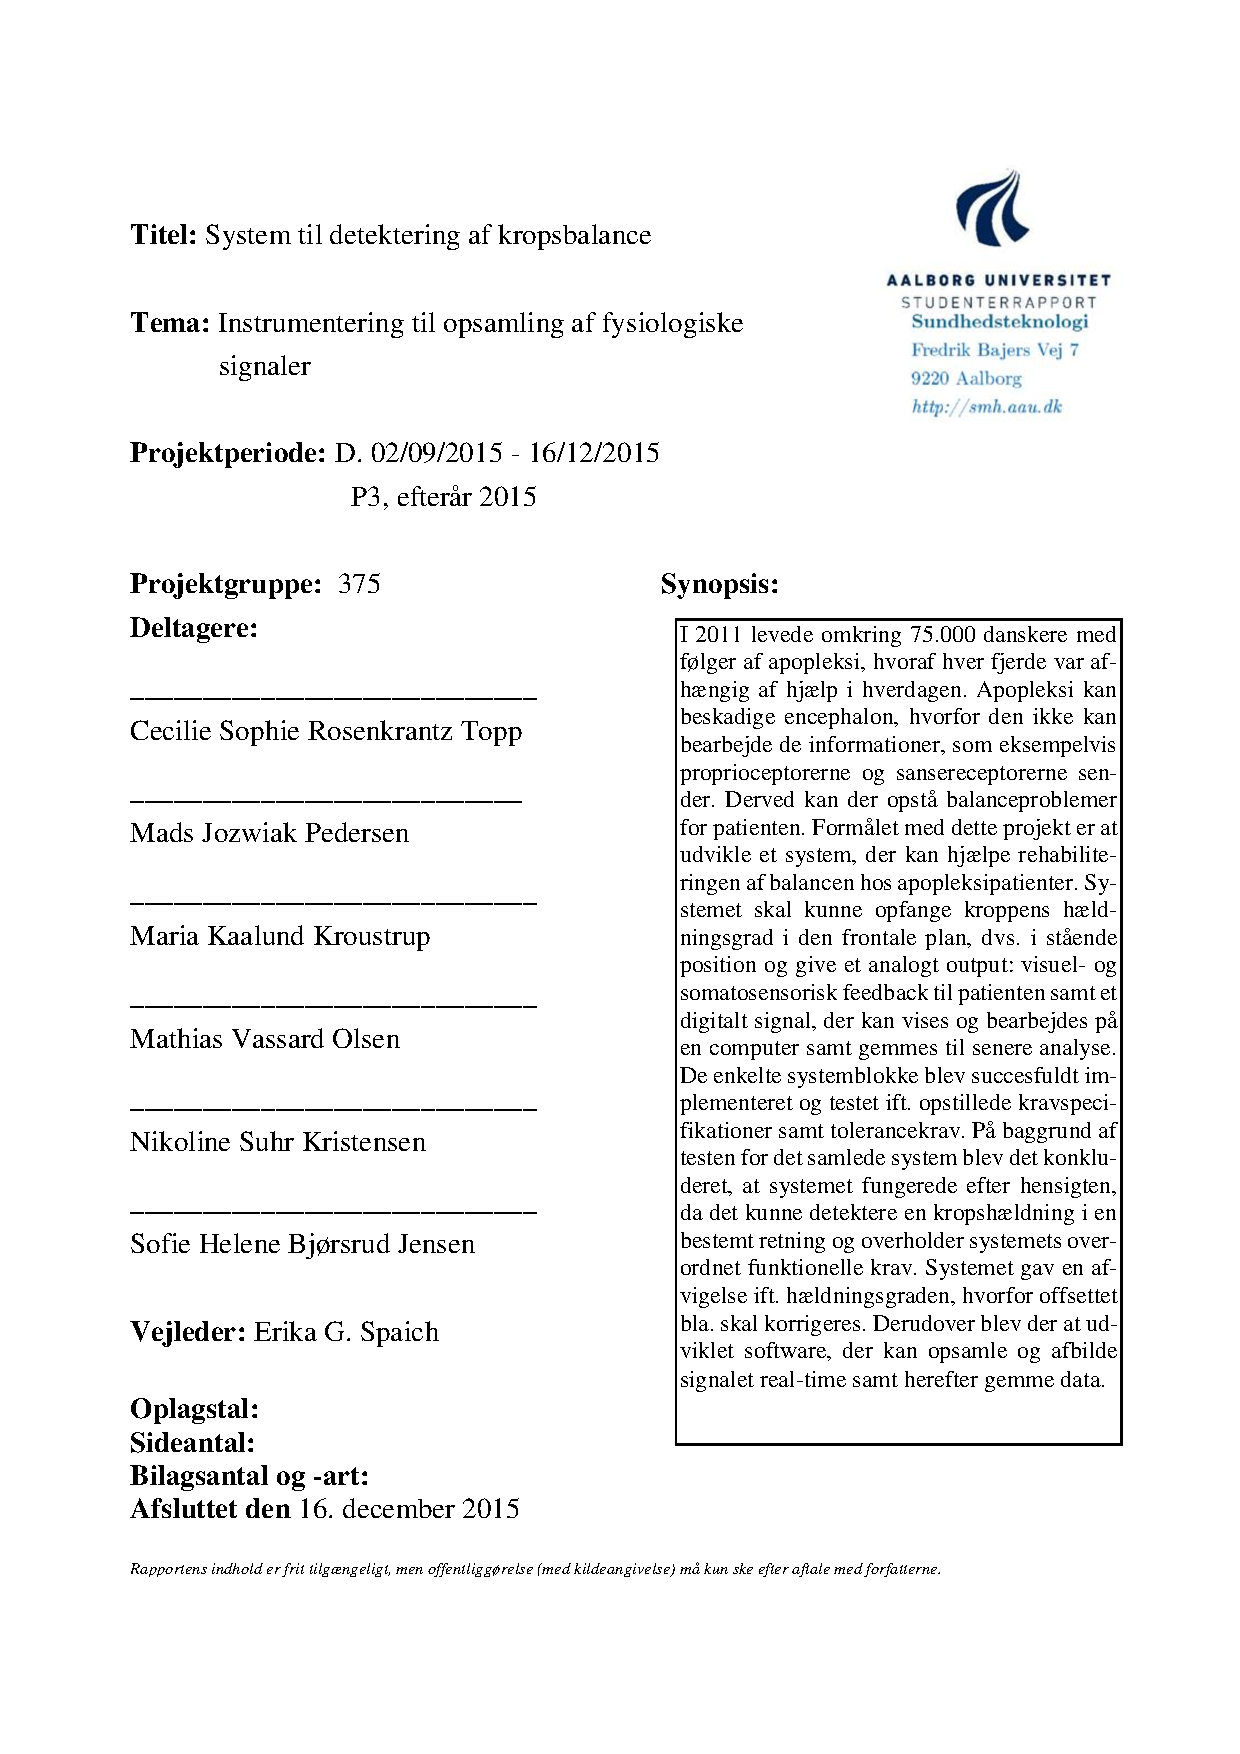
\includepdf[pages={1}]{rapportAfsnit/xFormaliteter/synopsis.pdf} 

% !TeX spellcheck = da_DK
\chapter*{Forord og læsevejledning}
\section{Forord}
Denne rapport er udarbejdet i forbindelse med et 3. semester projekt af studerende på Aalborg Universitet,  Sundhedsteknologi af gruppe 15gr375 i efteråret 2015. Ud fra projektets overordnede tema: "Instrumentering til opsamling af fysiologiske signaler" blev der heraf opstillet forskellige projektforslag. Denne rapport vil tage udgangspunkt i følgende projektforslag opstillet af Erika G. Spaich: "System til detektering af kropsbalance". Gruppens vejleder har under hele projektperioden været Erika G. Spaich.

Projektet rettes mod fagkyndigt personale, der beskæftiger sig med rehabilitering af apopleksipatienter og medstuderende på Aalborg Universitet, samt andre, der har interesse i emnet. 
Vi vil gerne takke vores vejleder Erika G. Spaich for vejledning og feedback igennem hele projektperioden. Derudover vil vi give en særlig tak til Jan Stavnhøj for hjælp og rådgivning til udarbejdelse af systemet samt Træningsenhed Vest Aalborg Kommune for at vi måtte komme og observere genoptræning af patienter med balanceproblemer. 

\section{Læsevejledning}
Projektrapporten er baseret på den problembaserede AAU-model. Selve rapporten er delt op i 4 kapitler, samt appendiks, således at første kapitel indeholder projektets initierende problem, der ligger til grund for problemanalysen. Andet kapitel indeholdende problemanalysen giver relevant viden om apopleksi og apopleksipatienternes følger, rehabiliteringsforløb og nuværende rehabiliteringsmuligheder, samt baggrundviden vedrørende teknologisk behandling af biologiske signaler.  Dette er efterfulgt af en projektafgrænsing samt problemformulering, der ligger til grund for problemløsningen. Problemløsningen beskrives i kapitel tre, indeholdende projektets praktiske del ift. at bygge et system til detektering af kropsbalancen. Herunder beskrives systemets kravspecifikationer samt systemdesign, herunder teori, simulering, implementering og test. I fjerde kapitel afsluttes rapporten med en evaluerende diskussion og konklusion af systemets funktion samt perspektivering ift. udvikling af systemet. Herefter findes litteraturlisten, samt appendiks, der henvises til som bilag A, bilag B osv. 

I rapporten benyttes Vancouver-metoden ved litteraturhenvisning, hvor anvendt litteratur tildeles fortløbende numre, således at den første reference i rapporten tildeles nummeret [1], den næste [2] osv. I litteraturlisten skrives den fulde reference, dvs. forfatter navn og årstal samt URL-kode hvis referencen er en hjemmeside, i den rækkefølge referencen anvendes i rapporten. Hvis referencen er placeret efter et punktum i en sætning tilhører referencen hele afsnittet, hvorimod er referencen placeret før et punktum tilhører referencen kun den pågældende sætning. Der der placeret flere referencer efter hinanden betyder dette, at der er anvendt flere referencer til den pågældende sætning eller afsnit. 

Derudover anvendes det amerikanske komma, når der i rapporten skrives tal, eksempelvis 12,500 og 2.4. Dvs. det amerikanske komma på dansk er et punktum og omvendt det amerikanske punktum på dansk er et komma.    

 \cleardoublepage

%the '*' allows the tableofcontents be excepted from the actual table of contents.
\tableofcontents*

%numbers the pages with Arabic numeral - starts from 1.
\mainmatter
\chapter{Indledning}
% !TeX spellcheck = da_DK
Apopleksi er pludselig opstået fokalneurologiske symptomer forårsaget af vaskulære forstyrrelser i hjernen, der kan forekomme pga. forhøjet blodtryk, diabetes eller rygning \cite{Sundhedsstyrelsen2009,Academic2015}. Apopleksi er den tredje største dødsårsag i Danmark og ca. 12.500 personer indlægges hvert år pga. sygdommen \cite{Hjernesagen2015a}. Andelen, der dør af hjerneskader, har været stagneret fra 2001 til 2011, hvor 14 \% døde inden for 30 dage \cite{Hjernesagen2015}. Derudover levede 75.000 danskere i 2011 med følger af apopleksi, og ud af disse er omkring hver fjerde person afhængig af hjælp for at kunne udføre dagligdagens gøremål \cite{Hjernesagen2015a}. Antallet af indlæggelsesforløb for mænd og kvinder stiger, når de bliver ældre end 65 år \cite{Sundhedsstyrelsen2011}.
Danskere der lever med følger og varige mén af apopleksi forventes at være stigende i takt med, at der kommer flere ældre \cite{Sagen2014}. Apopleksi er den sygdom, der kræver flest plejedøgn i sundhedssektoren. Ud fra et økonomisk perspektiv er det derfor dyrt for samfundet ift. omkostningerne til behandling, rehabilitering og produktivitetstab.  Udgifterne til sygdommen udgør 4\% af sundhedsvæsenets samlede udgifter, hvor direkte udgifter er estimeret til 2.7 milliard kroner om året \cite{Hjernesagen2015a, Kruuse2014}.
 
%I 2010 var der som sagt 18.041 indlæggelsesforløb forbundet med hjerneskade i Danmark, og det er langt fra alle, som slipper for varige mén heraf\cite{Sundhedsstyrelsen2011}. % gentagelse af det der skrevet før.
Følgerne af apopleksi opstår ofte pludseligt og kan både opleves som fysiske og mentale skader \cite{Muus2008}. Et af de hyppigste mén, som apopleksipatienter oplever, er neglekt. Patienter med neglekt er ikke opmærksomme på den ene side af kroppen \cite{Sundhed.dk}. Derudover opleves sensoriske- og motoriske skader herunder balanceproblemer. De nævnte følger har alle alvorlige konsekvenser for apopleksipatienters livskvalitet, da det bl.a. kan føre til  begrænsninger i hverdagen og i nogle tilfælde faldulykker. \cite{Muus2008,Nichols1997}

De fysiske- og mentale konsekvenser af sygdommen gør, det svært for en apopleksipatient at vende tilbage til sin normale hverdag. Problemer med balancen gør det f.eks. svært at udføre almindelige huslige pligter som rengøring og personlig pleje. \cite{Sundhedsstyrelsen2010} \\
Hjerneskadede patienter, heriblandt apopleksiramte, oplever nedsat livskvalitet pga. deres sygdom. Dette kan ses ved, at apopleksipatienter har dobbelt så stor selvmordsrate som baggrundsbefolkningen \cite{Sundhedsstyrelsen2010}. I en kvantitativ undersøgelse nævner 16\% af apopleksipatienter, at deres livskvalitet er dårlig	\fxnote{46\% nogenlunde, 38\% god} \cite{Sundhedsstyrelsen2010}. Den nedsatte livskvalitet kan føre til vanskeligheder senere i livet \fxnote{Måske skrive hvorfor}. En forbedret livskvalitet kan skabes ved hurtigere rehabilitering eller forbedret kropslige funktioner, som den apopleksiramte mistede ved hjerneskaden. \cite{Sundhedsstyrelsen2010}

For at patienterne opnår den bedst mulige behandling og rehabilitering er det afgørende, at der er et fungerende sammenspil mellem kommuner, sygehuse og praktiserende læger. Apopleksipatienter er krævende ift. rehabilitering pga. omfattende følger efter hjerneskaden. \cite{Sundhedsstyrelsen2010} Det er derfor vigtigt, at fokusere på patienternes rehabilitering for at kunne genoptræne de forskellige fysiske- og mentale mangler de oplever i dagligdagen samt give dem større livskvalitet. 

%Akut behandling og rehabilitering afhænger organisatorisk af hinanden, da sammenspillet mellem kommuner, sygehuse og praktiserende læger er afgørende. % Apopleksi har omfattende og alvorlige konsekvenser og der er derfor brug for involvering fra flere sundhedsprofessionelle områder.\cite{Sundhedsstyrelsen2010}
%De omfatende og alvorglige konsekvenser samt sammenspillet mellem sundhedsområder og rehabilitering er bl.a. det, som gør, at apopleksi er omkostningsfuldt for samfundet.\cite{Sundhedsstyrelsen2010} \\
%Apopleksi påvirker patienters livskvalitet og identitet, da det er svært for patienterne at forholde sig til sygdommen og derved påvirker deres humør, personlighed, færdigheder og sociale relationer. Det er derfor vigtigt at genoptræne patienterne ved at rehabilitering for, at de kan genfinde eller forbedre deres tabte funktioner, f.eks. ved brug af teknologier, som på denne måde er med til at genoprette identitet samt forbedre livskvaliteten for patienten.\cite{Sundhedsstyrelsen2010} 

%Det vil derfor kunne forventes, at der er flere, som kommer ud for en hjerneskade og vil have varige mén herefter, hvilket gør det vigtigt at fokusere på rehabiliteringen for at kunne genoptræne de forskellige kropslige- og mentale mangler.

%%%%%%%%%%%%%%%   Marias foreslag til indledning
%Det kræver samarbejde fra flere professionelle plejepersonale som kommuner, sygehuse og praktiserende læger for at give patienten den rette rehabilitering, da apopleksi patienter er omfattende og kan have alvorlige konsekvenser. Dette gør også at apopleksi er omkostningsfuldt for samfundet. 
% !TeX spellcheck = da_DK
\section{Initierende problem}
Hvilke fysiologiske konsekvenser kan apopleksi have for patienten, og hvad er rehabiliteringsmulighederne for en patient med balanceproblemer? 

%%%%%%%%%%%%%% FORESLAG TIL ANDRE INITIERNEDE PROBLEMER, DER ER MERE PROBLEMORIENTERET %%%%%%%%%%%%%
% 

\chapter{Problemanalyse}
\section{Apopleksi}

Et apopleksi tilfælde kan være forårsaget af enten en blodprop i hjernen (iskæmisk) eller hjerneblødning (hæmoragisk).
Apopleksi er af World Health Organization (WHO) defineret som pludseligt opstået fokale neurologiske symptomer pga. forstyrrelser i hjernens blodcirkulation, der varer mere end 24 timer eller fører til døden[1]. Hvis varigheden er under 24 timer, betegnes det som transitorisk cerebral iskæmi (TCI), hvor de fleste tilfælde varer under 1 time[2] uden permanent hjerneskade [3].

(Billeder)

Iskæmisk apopleksi forekommer hyppigst%ift. hvad? 
[2] og opstår, når en hjernearterie blokeres af en blodprop (infarkt), der stopper tilførslen af blod til et bestemt område i hjernen, hvilket ses på figur xx. Infarkterne dannes primært pga. åreforkalkning enten ved en trombe, der dannes på stedet, eller emboli fra hjertet. Nervecellerne skades efter få minutter pga. stoppet blodtilførsel og vil gå tabt [5].

Hæmoragisk apopleksi skyldes hovedsageligt forhøjet blodtryk eller i sjældnere tilfælde bristede svagheder på arterier (aneurismer) eller misdannede kar[5]. Hæmoragisk apopleksi opstår, når en hjernearterie brister og lækage af blod danner en blodansamling (hæmatom), der beskadiger det omkringliggende væv og forøger trykket i hjernen, hvilket ses på figur xx. Blødning i selve hjernen (intracerebral hæmoragi) kommer af forhøjet blodtryk, der danner et pres på de små arterier, som får dem til at briste[4] og forekommer i 10-12\% af tilfældene[2]. %ift. hvilke tilfælde? 
Blødning i rummet mellem de to hjernehinder (subaraknoidalrummet) skyldes bristning af et aneurisme på en pulsåre i hjernen [5] og forekommer 3-5\% af tilfældene[2]. Symptomerne ved subaraknoidalblødning er generel tab af hjernefunktion, da der forekommer et øget pres på hjerneskallen, hvorimod ved intracerebral hæmoragi er hæmatomet lokaliseret et bestemt sted i hjernen og forårsager nedsat funktion ved én bestemt hjernefunktion[4]. 

% WHO - find en dansk difination istedet.
% Fjern paranteserne - skrev enten det rigtige ord først eller lav en anden måde at skrive det på.
% Mangler lidt en forklaring på, hvordan og hvorfor apopleksi det opstår. Man kan godt uddybe mere i det, der allerede er skrevet.
% Når der er bygget mere på, kan man godt lave nogle forskellige overskrifter.
% Fakta omkring, hvad der er årsagen til apopleksi - hjertesagen har nogle forksellige info om det. Fakta om apopleksi.
% !TeX spellcheck = da_DK
\section{Diagnosticering}

Når en patient med apopleksi indlægges, er grundig undersøgelse nødvendig for at identificere, hvilken form for apopleksi der er tale om. Dette trin er afgørende for det efterfølgende forløb, da behandling samt rehabilitering planlægges herefter. \cite{Sundhedsstyrelsen2009}

\subsection{Anamnese}
For at blive bekendt med patientens egen subjektive vurdering af det hidtidige sygdomsforløb, optager lægen en anamnese. Her skal sygdomsforløbet  beskrives detaljeret, og der skal desuden spørges ind til faktorer, som kan have været medvirkende til udviklingen af apopleksi såsom livsstil og sygdomme, herunder f.eks. diabetes og hjerteproblemer. \cite{Sundhedsstyrelsen2009}

\subsection{Klinisk undersøgelse}
Den kliniske undersøgelse udføres for at vurdere hvor alvorligt et sygdomstilfælde, der er tale om. Undersøgelsen udføres ud fra en standardiseret skala, da dette gør det muligt for andre læger at undersøge patienten på samme måde senere i forløbet. Resultatet af undersøgelsen er en samlet score udregnet fra resultatet af de enkelte undersøgelser. Det er således muligt at vurdere om der sker fremskridt hver gang undersøgelsen foretages. \cite{Sundhedsstyrelsen2009}

Der findes flere forskellige skalaer, som lægen kan anvende til at foretage den kliniske undersøgelse, herunder Scandinavian Stroke Scale, European Stroke Scale og Hemisperic Stroke Scale. Fælles for skalaerne er, at de alle undersøger både bevidsthedsniveau samt motoriske og kognitive egenskaber hos patienten \cite{Center, Centera, Centerb, Centerc}. I den danske sundhedssektor benyttes Scandinavian Stroke Scale, dette blev besluttet i Det Nationale Indikatorprojekt for apopleksi \cite{Apopleksi2009}. F.eks. har Region Syddanmark derudover forskellige retningslinjer for hvilken skala, der skal benyttes i et apopleksi forløb \cite{Syddanmark}. Alle apopleksi patienter, der bliver indlagt med mulig akut apopleksi eller TCI, skal have en score på Scandinavian Stroke Scale. Herefter benyttes National Institute of Health Stroke Scale hvis patienten skal have trombolysebehandling. Barthel Scale anvendes hvis patienten sendes til videre rehabilitering og beskriver patientens funktionsniveau i forhold til almindelige dagligdags funktioner. Til sidst benyttes Modificeret Rankin Scale til at give en beskrivelse af graden af handicap. \cite{Syddanmark}

\subsection{Videre undersøgelser}
Ved den videre undersøgelse vil der udføres en scanning for at undersøge, om patienten er ramt af en hjerneblødning eller en blodprop. Scanningen laves desuden for at lokalisere det ramte område. Enten udføres der en scanning af typen CT eller MR afhængigt af, hvad der er mest hensigtsmæssigt i den givne situation. \cite{Sundhedsstyrelsen2009} %CT-scanning udsender røntgenstråligen, hvilket optages i vævet på forskellige måder. Udfra dette beregner en computer tværsnitsbilleder af kroppens indre \fxnote{https://www.cancer.dk/hjaelp-viden/undersoegelser-for-kraeft/scanninger-billedundersoegelser/ct-scanning/}. Modsat anvendes der ved MR-scanning et kraftigt magnetfelt som sender radiobølger ind i kroppen. Derved registres et ekko og computeren kan derefter beregne et detaljeret billede af kroppens indre organer. 
CT-scanning anvendes f.eks. til undersøgelse af åreforkalkning og indre blødninger, hvor MR-scanning bruges til at undersøge sygdomme i nervesystemet f.eks. i hjernen \cite{Hansen2015,Ammundsen2015}.\\
Det skal derfor vurderes, hvilken form for scanning der skal anvendes ud fra forskellige kriterier, herunder lægens mistanke om, hvilket område af hjernen der er ramt, samt hvor længe symptomerne på apopleksi har optrådt. I visse tilfælde kan lægen vælge at anvende begge scanningstyper.  
Derudover skal patientens blodtryk måles jævnligt i den akutte fase for at sikre, at det falder gradvist til et normalt niveau i løbet af nogle timer til et døgn. Hvis blodtrykket pludselig falder meget, kan dette være et udtryk for en blodprop i hjertet. Det er derfor afgørende at følge udviklingen med jævnlige blodtryksmålinger. \cite{Sundhedsstyrelsen2009}
\\
Under forløbet bør andre faktorer også kontrolleres, herunder lungefunktion, blodsukker og kropstemperatur. Disse faktorer kan enten give information om apopleksien, eller de kan være væsentlige for patientens fremtidsprognoser og følger efter sygdomsforløbet. \cite{Sundhedsstyrelsen2009}
\\

% [1] Sundhedsstyrelsens rapport
% [2]http://www.strokecenter.org/professionals/stroke-diagnosis/stroke-assessment-scales/
% [3]http://www.strokecenter.org/wp-content/uploads/2011/08/hemispheric.pdf
% [4]http://www.strokecenter.org/wp-content/uploads/2011/08/scandinavian.pdf
% [5]http://www.strokecenter.org/wp-content/uploads/2011/08/European_Stroke_Scale.pdf
% [6]http://www.dsks.dk/filer/hoeringssvar/referenceprogram_for_behandling_af_patienter_med_apopleksi.pdf
% [7] http://ekstern.infonet.regionsyddanmark.dk/Files/dokument90214.htm
% [8] https://www.sundhed.dk/borger/sygdomme-a-aa/hjerte-og-blodkar/sygdomme/apopleksi/apopleksi-blodprop-eller-bloedning-i-hjernen/
% [9] http://academic.eb.com.zorac.aub.aau.dk/EBchecked/topic/569347/stroke
% [10] http://www.netdoktor.dk/sygdomme/fakta/blodprophjerne.htm
% !TeX spellcheck = da_DK
\section{Behandlinger}
Når en patient rammes af apopleksi, er det vigtigt at komme i behandling hurtigst muligt. Ved ankomst på sygehuset foretages der en scanning af encephalon for at undersøge, hvorvidt det er iskæmisk eller hæmoragisk apopleksi. Hvis hæmoragisk apopleksi findes der endnu ingen akut behandling, der kan stoppe blødningen.\cite{Soenderborg2013} Hvorimod ved akut iskæmisk apopleksi, hvilket vil sige at symptomerne er til stede inden for fire en halv time, anvendes blodpropopløsende medicin. Ved hurtig behandling vil det være muligt at opløse blodproppen. I andre tilfælde fjernes blodproppen ved brug af et tyndt kateter, som indføres gennem arterien op til encephalon. Derudover anvendes blodfortyndende medicin for at undgå nye tilfælde af apopleksi. \cite{Hjerteforeningen2014, Kruuse2014a} 

%\subsection{Akut behandling}
%Ved mistanke om iskæmisk apopleksi er det vigtigt, at der tages kontakt til sygehuset omgående. Patienten bliver her undersøgt ved blodtryksmåling, blodprøver, neurologisk undersøgelse og scanning af encephalon. Dermed kan det udelukkes om der er eventuelle blødninger eller andre årsager til funktionstabet. Dette  sikrer, at patienten får den rette behandling. I tilfælde af blodprop igangsættes en behandling med blodpropopløsende eller blodpropshæmmende medicin. \cite{Hjerteforeningen2014, Kruuse2014a} 
%
\subsection{Trombolyse}
Standardbehandling for blodpropper har siden år 2006 været trombolyse. Selve behandlingen foregår ved, at der sprøjtes blodpropopløsende medicin ind i en arterie, ofte i armen, hvorefter blodproppen opløses. Denne behandling skal helst foregå seks timer efter blodproppens forekomst og senest 12 timer efter, da behandlingen ikke vil have nogen indvirkning efter længere tid. Hurtig behandling vil betyde at flere områder af encpehalon vil kunne reddes. Dermed vil patientens fremtidige livskvalitet forbedres. Trombolysebehandlingen finder sted på 12 sygehuse fordelt over de fem regioner. En risiko ved behandlingen kan være blødninger grundet den blodpropopløsende medicin. \cite{Hjernesagen2015b}

\subsection{Forebyggelse}
En væsentlig del af behandlingen er forebyggelse, da risikoen for en ny blodprop er betydelig. Til forebyggelse anvendes antikoagulationsbehandling, som er en behandling med blodfortyndende medicin. Normalt har kroppen sit eget koagulationsssystem som får blodet til at koagulere. Derudover medvirker koagulationssystemet også til at opløse evt. blodpropper i det kardiovaskulæresystem. For apopleksipatienter fungerer koagulationssystemet ikke optimalt, hvilket gør det nødvendigt at behandle med antikoagulation. Dette hæmmer blodets evne til at koagulere, hvilket modvirker dannelsen af blodpropper. Der findes to former for antikoagulationsbehandling, warfarin og nyre orale antikoaglulantia. Den primære forskel mellem de to mediciner er, at der ved behandling med nyre orale antikoaglulantia ikke kræves kontrol ved blodprøver.\cite{Kjaergaard2015}

%[1]http://www.hjerteforeningen.dk/alt-om-dit-hjerte/hjerte-kar-sygdomme/apopleksi/
%[2]http://www.hjernesagen.dk/om-hjerneskader/behandling/trombolyse
%[3] https://www.sundhed.dk/borger/sygdomme-a-aa/hjerte-og-blodkar/sygdomme/apopleksi/behandling-ved-apopleksi/
%[4]https://www.sundhed.dk/borger/sygdomme-a-aa/hjerte-og-blodkar/sygdomme/behandlinger/antikoagulationsbehandling-blodfortyndende-medicin/
\input{rapportAfsnit/cProblemanalyse/Foelger}
\section{Balance}
Efter et apopleksi tilfælde kan patienterne have balance problemer, hvilket kan give farlige situationer, hvor patienten har risiko for faldulykker. Balancen er styret af forskellige organer i kroppen. Organerne styrer balancen ved at bruge sansereceptorer. Sansereceptorer er en bestemt slags celler, hvis funktion består i at sende informationer til det centralnervesystem og hjerne vedrørende kropsbalancen. Sansereceptorerne opfanger sanseindtryk og videregiver informationen til områder i cerebral cortex, cerebellum og til centre i hele hjernestammen. Disse områder bearbejder informationen, for at konkludere den fysiske position af kroppen og dens lemmer. [1]\\

Balancen er i virkeligheden et komplekst system, da flere forskellige kropssystem samarbejder i forhold til at sende indtryk til hjernen, hvor de bearbejdes. Når hjernen har bearbejdet indtrykkene udsendes nerveimpulser til skeletmuskulaturen om at foretage jævne og koordinerede bevægelser, hvorved kropsbalancen opretholdes. [1] For apopleksipatienter opleves der ofte problemer med balancen. Patienterne hænger mod deres syge og svage side uden de er opmærksomme på det, da deres balance ofte er nedsat eller slet ikke funktionsdygtigt. [2] 

De sansereceptorer, som indvirker til at opretholde balancen, i form af at holde kroppen i en lodret position, og korrigere eventuelle kropshældninger er placeret i ørerne og øjnene.  [1]

\subsection{Øret} \fxnote{Afsnittene skal muligvis ændres til latinske betegnelser}

Øret består overordnet af tre dele. Det ydre øre, mellemøret og det indre øre. Det er i det indre øre, som er med til at kontrollere balancen, da det indeholder de receptorer, som består af hårceller, som reagere på forskellige stimuli og er med opretholder balancen i kroppen. Det indre øre er som en knoglelabyrint, hvor der findes et netværk af sammenhængende væskeholdige kanaler, som er indkapslet i knogle. Det er i disse kanaler receptorerne sidder. Det indre øre kan yderligere opdeles i tre underdele: vestibulen, øresneglen og buegangen. Vestibulen består af et par membransække: Sacculen og utriclen. Disse membransække opfanger sanseindtryk vedrørende tyngdekraft og lineærer accelerationer. \fxnote{Ved ikke om der skal skrives om øresneglen, da den ikke har noget med balancen at gøre, men derimod hørelsen} Buegangen består af væskefyldet knoglekanaler og her sidder også de receptorer, som opfanger stimuli omkring hovedets bevægelse og viderebringer information om hovedet rotationer, og hvor hurtig bevægelsen foregår. Receptorerne består af hårceller, som sidder i buegangenes ampulla, som er placeret, hvor buegangene er forbundet til utriculen. I utriculen og sacculen sidder der øresten, som indeholder hårceller, som opfanger information vedrørende hovedets bevægelse i forhold til tyngdekraften. Dette sker når hovedet bevæger sig, sættes væsken i kanalerne i bevægelse. Væskebevægelser i den ene retning stimulerer hårcellerne, mens bevægelser i den modsatte retning forhindrer dem. De forskellige buegange stimuleres af forskellige hovedbevægelser, for på den måde at få bedst mulig information. Informationen sendes via vestibulocochlearnerven, som sender information til hjernen i områder i pons og medulla oblongata vedrørende balance og hørelse. [1]    

\fxnote{Indsæt illustration af ørets anatomi, hvor ampulla med hårcellerne kan ses! Kunne være den fra Martini 9th side 577 eller side 579 }

\subsection{Øjet og det visuelle}
Øjnene og synet har den funktion at holde hjernen informeret om kroppens balance og generel orientering, ved at give et indtryk af, hvordan kroppen og dens lemmer er placeret i forhold til omgivelserne. Det er fotoreceptorer, som er placeret i nethinden \fxnote{retina}, der udgøre den inderste del af øjet. Nethinden består af et ydre lag, som er pigmentdelen og en indre neural del. Den neurale del indeholder lysreceptorer, støttende celler og neuroner, der udfører behandler visuel information. Pigmentdelen har den funktion at absorberer lys, som passerer gennem den neurale del og gør at lyset ikke har mulighed for at reflektere tilbage til den neurale del. Foto- og lysreceptorerne konverterer lyset fra omgivelserne til elektrisk nervesignal, som sendes via synsnerven til den visuelle cortex i storhjenehemisfæren, hvor informationen bearbejdes. [1]  

\fxnote{Muligvis indsæt illustration af øjets anatomi f.eks. Martini 9th side 557}

\subsection{Proprioceptorerne og skeletmuskulaturens indvirkning på balancen}
Proprioceptorer findes i skeletmuskulaturen og er receptorer, der monitorer leddenes position, spændinger i sener og ledbånd, samt muskelkontraktionernes tilstand. Informationerne som opfanges sendes via nervesignal til rygmarven og herfra igennem centralnervesystemet til cerebellum. Proprioceptorer bliver inddelt i tre overordnet grupper: muskelspindlere, golgi sene organer og receptorer i ledkapsler. [1]

Muskelspindlere er den gruppe, som styre og kontrollerer ændringer i muskellængden og kan udløse en strækrefleks, som derved regulerer skeletmuskulaturens længde. Til muskelspindlerne er der forbundet sensoriske og motoriske nerver. Den sensoriske nerve er forbundet central på muskelspindleren, hvor den sender sensoriske impulser.  (Se Martini 9th side 438 under "monosynaptic reflexes")  

Golgi seneorganer (Se Martini 9th side 501 under 15-3 propriocetor)
Receptorer i ledkapsler (Se Martini 9th side 501 under 15-3 propriocetor)

\fxnote{Mangler: Det sidste afsnit propriocerptorerne mangler at blive skrevet helt færdigt. Derudover kunne man have en konklusion hvor der blev kigget på sammenspillet mellem de forskellige dele der har med balancen at gøre. Vi kunne også godt have skrevet til hvilke nervesystemer der sig af signalerne i de forskellige organer. Så skal lange sætninger osv. lige rettes igennem.}


[1] – Martini, Frederic H and others. Fundamentals of Anatomy & Physiology (Kapitel:13, 14, 15, 17 ). 2012. Pearson. 
[2] - Karnath2003


% !TeX spellcheck = da_DK
\section{Rehabilitering}
Når selve slagtilfældet er stabiliseret og behandlet, er det essentielt, at rehabiliteringen af en apopleksipatient indfindes hurtigst muligt - gerne en til to dage efter slagtilfældet. I Danmark dækker rehabilitering af en patient med apopleksi områderne: direkte træning af funktioner, ufrivillig reorganisering af hjernen netværk, kompenserende strategier, ændringer i miljø, social og psykologisk støtte. Genoptræningen omhandler dog ikke kun træning med en ergo- eller fysioterapeut, da plejepersonale til dagens almindelige gøremål også essentiel. Patientens daglige rutiner kan være gået tabt under slagtilfældet, hvorfor det er vigtigt, at få patienten tilbage i sit vante miljø. Plejepersonale skal hjælpe patienten til at genfinde denne rytme og hjælpe patienten til eventuelt at udføre dagligdags ting på en ny måde. Det kan ske, at patienten ikke længere er i stand til at beherske begge sine hænder til en opgave, hvorved plejepersonalet skal bistå patienten i indlæringen af kun at benytte en hånd.

Motoriske og sensoriske funktionsproblemer kan lede til balancebesvær for patienten i både siddende, stående og gående stilling. Der er afprøvet adskillige farmakologiske midler og behandlingsstadegier for at forbedre hjernens rehabilitering og motoriske funktioner. F.eks. er der afprøvet, at tildele apopleksipatienter det antidepressive middel fluoxetin i kombination med fysioterapi. Derudover er kortikal stimulation afprøvet, hvor området af hjernen, som kontrollerer motorstyring, modtager elektriske impulser fra en implanteret anordning. Denne mulighed har haft blandede succesoplevelser, men er udelukkende afprøvet på patienter, der har oplevet et alvorligt slagtilfælde. \cite{Academic2015}
  
Apopleksi patienten skal i samarbejde med lægen, sygeplejersken og andet hjælpepersonale opstille nogle mål for sin rehabilitering. Målene skal hverken være for svære eller for lette, så patienten ikke mister sin motivation til genoptræningen. \cite{Kruuse2015}

\subsection{Forløbsprogram for rehabilitering} 
Sundhedsstyrelsen har udarbejdet et forløbsprogram for rehabilitering af patienter med erhvervet hjerneskade. Forløbsprogrammet strækker sig fra at patienten erhverver hjerneskaden til at patienten har opnået bedst mulig funktionsevne, hvorefter der udføres kontrol og vedligeholdelse af funktionsevnen. Tidsperioden af rehabilitering varierer ift. hjerneskadens sværhedsgrad, samt sværhedsgraden af funktionstabet. %dog kan perioden vare flere år.  
\cite{Sundhedsstyrelsen2011a}

Forløbsprogrammet er essentielt i forhold til at kunne give patienten den korrekte rehabilitering. Patienterne har forskellige behov og er afhængige af hjælp fra plejepersonale. Deruodver kræves der forskellige former for teknologi i de forskellige faser. Det vil derfor være oplagt at undersøge, hvilken form for rehabilitering der er at foretrække i de enkelte faser som ses på \figref{firefaser}.

\begin{figure}[H]
	\centering
	\includegraphics[scale=0.6]{figures/bProblemanalyse/flowdiagram_faser1.png}
	\caption{På figuren ses et overblik over de fire faser, som patienter med apopleksi skal igennem i forløbsprogrammet for rehabilitering \cite{Sundhedsstyrelsen2011a}} 
	\label{firefaser}
\end{figure}

\subsubsection{Den første fase}
Som det vises på \figref{firefaser} afspejler første fase den del af forløbsprogrammet som foregår på sygehusets apopleksiafdeling. På apopleksiafdelingen foretages primært akut behandling for at begrænse skaderne. Når patientens sikkerhed er sikret og skaderne er begrænset påbegyndes den tidlige rehabilitering. Under den tidlige rehabilitering giver en speciallæge i neurologi en vurdering af patientens rehabiliteringsbehov. Derudover bliver patienterne overvåget i forhold til bevidsthed, ændringer og amnesi samt foretaget vurderinger af basale fysiologiske funktioner. Samtidig bliver der iværksat træning i diverse bevægelsesfunktioner, basale egenskaber og kommunikationsfunktioner. Patienterne gennemgår også en tidlig behandling og diagnostik for at undersøge komplicerende tilstande, som f.eks. vaskulære hændelser, blodpropper i ben og lunger og smerter. Patienterne vurderes i denne fase af fagkyndigt personale som ergoterapeut, fysioterapeut og audiologopæd \fxnote{høre og talepædagog}. Disse er med til, at sikre, at patienten udfører træningen korrekt i forhold til stilmulering og træning af bevægelsesfunktioner, taletræning og udførsel af basale daglige aktiviteter.\cite{Sundhedsstyrelsen2011a}

\subsubsection{Den anden fase}
Det fremgår af \figref{firefaser}, at patienten i den anden fase gennemgår rehabilitering på sygehuset, hvor der er fokus på de skadede funktioner. Ligeledes bliver patienten på samme måde som i fase et undervist af fagkyndigt personale. Hvorefter patientens behov for rehabilitering og rehabiliteringens udvikling vurderes. Patienterne bliver i denne fase udredet i forhold til funktionsevne, mentale funktioner, bevægelsesfunktioner herunder bevægelse og mobilitet i led, knogler, reflekser og muskler samt rehabilitering med henblik på daglige aktiviteter. Hvis patienten vurderes til at have en stabil udvikling i rehabiliteringsprocessen, vil patienten blive udskrevet og påbegynde fase tre. \cite{Sundhedsstyrelsen2011a}


\subsubsection{Den tredje fase}
I den tredje er patienten udskrevet fra sygehuset. Derved foregår rehabilitering som ambulant rehabilitering og selvstændig træning, som det fremgår af \figref{firefaser}.  Selve rehabiliteringen i tredje fase er bygget op ud fra rehabiliteringsforløbet i den anden fase. Det afgørende for den tredje fase er, hvorvidt patienten skal vedblive rehabilitering på sygehuset eller henvises til de kommunale rehabiliteringscentre. Dette afgøres på baggrund af observationer foretaget i anden fase. Den selvstændige træning kan for patienter med neglekt og balanceproblemer være en udfordring ift. bevægelsesmønstre og kropsholdning. \cite{Sundhedsstyrelsen2011a}

\subsubsection{Den fjerde fase}
Det fremgår på \figref{firefaser}, at fjerde fase er den afsluttende fase for behandlingsforløbet. Patienterne går stadig til kontrol og vedligeholdelse for at sikre, at rehabiliteringens udvikling er stabil. Det kan i sidste ende have betydning for, hvor lang tid det tager for patienten at generhverve sine tabte funktioner. Den fjerde fase varierer derfor fra patient til patient alt efter udviklingen af rehabiliteringen.\cite{Sundhedsstyrelsen2011a} \\

\subsection{Organisatorisk}
Sygehusvæsenet, almen praksis og kommuner har opgaver i alle faser, dog i varierende grad. Således har sygehuset flest opgaver i fase I og II, mens kommunen og almen praksis har flest opgaver i fase III (og IV) \cite{Sundhedsstyrelsen2011a}.

%\section{Organisatorisk}
%I sundhedssektoren arbejder de forskellige organisatoriske aktører på tværs af hinanden. Der er således et samarbejde mellem syghuse, kommuner og praktiserende læger. Dette samarbejde skal ske både internt på syghusene, på afdelingerne og kommunalt mellem forvaltningerne \cite{Sundhedsstyrelsen2010}. Samspillet mellem aktørerne er vigtigt, da patienter med hjerneskade berører flere afdelinger. De har derfor brug for involvering af flere sundhedsprofessionelle grupper under behandling og rehabilitering på grund af de omfattende og alvorlige konsekvenser.

%De ovennævnte aktører er de organisatoriske enheder, der har en central rolle i forløbet. Det er ikke muligt at fastlægge en egentlig organisering af hjerneskaderehabiliteringen i Danmark, da sammenspillet mellem de forskellige aktører er meget flydende og forskellige alt efter hvor i landet man befinder sig og hvor omfattende hjerneskaden er. Denne forskel opleves regionalt, hvor behandling og rehabilitering enkelte steder foregår på få af sygehusets afdelinger, mens patienter andre steder behandles på et rehabiliteringssygehus, efter den akutte behandling er foretaget.\cite{Sundhedsstyrelsen2010}

%I starten af behandlingssforløbet sendes patienterne til neurologiske, geriatriske, neurokirurgiske og medicinske afdelinger på sygehuset. Som tidligere nævnt inddeles patienterne efter sværhedsgrad af hjerneskaden, hvor de sværest ramte, som er patienter med traumatisk hjerneskade og tilgrænsede lidelser, vidererstilles til Hammel og Hvidovre. Rehabiliteringen kan også ske på rehabiliteringsafsnittene på landets sygehuse.
%Det primære ansvar ligger hos kommunerne i form af genoptræningsplanens afdækning af rehabiliteringsbehov, dvs. at kommunerne holder øje med om dette foregår i praksis, herunder bl.a. patientens genoptræningsbehov. Kommunen har derudover mulighed for at henvise patienterne til dens egne tilbud, samt at henvise til private.\cite{Sundhedsstyrelsen2010} 

%Afslutningsvis gennemgår patienterne et langt og forskelligt behandlingsforløb alt efter hjerneskadens omfang. Forløbet indebærer et samarbejde mellem de forskellige aktører. Efter behandlingen står kommunerne, som førnævnt, for det primære ansvar i forhold til rehabilitering og henvisning for patienten\fxnote{hvor kommer denne info fra?}.



% I første og anden fase af rehabiliteringsforløbet bliver patienten undervist og overvåget af fagkyndigt personale. Dette gøres for at sikre, at patienten udfører træningen korrekt f.eks. med bevægelsesmønstre, og korrigere patienten til at bevægelsen og øvelserne udføres korrekt. Dette er vigtigt, da patienten, som sagt i tredje fase, selv skal foretage den nødvendige træning og dermed har fornemmelse af, hvordan træningen udføres korrekt ift. bevægelsesmønstre og kropsholdning. Dette kan midlertidig være en udfordring for apopleksipatienter med neglekt, da de kan have problemer med balancen og opmærksomheden på kroppen. Patienten går derfor stadig til kontrol og vedligeholdelse for at sikre, at rehabiliteringens udvikling er stabil. Det kan i sidste ende have betydning for, hvor lang tid det tager for patienten at generhverve sine tabte funktioner. Den tredje fase varierer derfor fra patient til patient alt efter udviklingen på rehabiliteringen. \cite{Sundhedsstyrelsen2011a}
% !TeX spellcheck = da_DK
\subsection{Nuværende metoder til rehabilitering}

Inden patienten udskrives fra sin behandling skal der fra sundhedssektorens side være udarbejdet en genoptræningsplan. I denne plan besluttes det hvilken form for rehabilitering og teknologi patienten skal benytte sig af. \cite{Sundhedsstyrelsen2011a} \\
Der findes flere forskellige metoder og teknologier til at hjælpe med balance og gangproblemer. Disse omfatter: Platform feedback, fokuseret gangtræning, konditionstræning, auditorisk rytmestøtte, elektromekanisk fysioterapistøttet gangtræning, opgavespecifik repetitiv træning, spejlterapi, programmer til motorisk visualisering og passiv sensorisk stimulation. \cite{Sundhedsstyrelsen2011a}\fxnote{dette skal laves om til punktform.} \\
Platform feedback er en biofeedback metode, hvor patienten står på en platform. Platformen vil herefter måle hvor meget patienten svajer \fxnote{(centre of pressure)}. Når platformen har målt svajningen af patienten, kan denne enten få visuel eller auditiv feedback. Feedbacken skal gøre patienten mere opmærksom på, hvor meget kroppen svajer, hvilket gør det muligt at opretholde en stående position.%[1]
Denne form for teknologi benyttes særligt i de tidlige faser af rehabiliteringen\cite{Sundhedsstyrelsen2011a}. \\
Det er med høj evidens blevet påvist, at fokuseret gangtræning medfører en moderat grad af bedringen på gangfunktionen hos apopleksiramte\cite{Sundhedsstyrelsen2010}. Derudover er det også vist, at konditionstræning kan være med til at forbedre gangfunktionen\cite{Sundhedsstyrelsen2010}. \\
Auditorisk rytmestøtte er en metode, hvor patienten lytter eller udfører handlinger til en form for musik. Det mest centrale ved musikken er rytmen, der findes i den.%[2] 
Det er vist, at denne metode kan øge både ganghastigheden, skridtlængden og gangsymmetrien \cite{Sundhedsstyrelsen2010}. \\
Ved elektromekanisk fysioterapistøttet gangtræning benytter fysioterapeuten sig af en maskine til hjælp af patientens gang. Maskinen består af enten et robot-drevet exoskelet eller to drevne mekaniske plader, der simulerer gang hos patienten. %[3] 
Denne form for metode har vist at kunne øge skridthastighed, skridtlængde og skridtsymmetri \cite{Sundhedsstyrelsen2010}. Denne metode benyttes til patienter med svært nedsat gangfunktion, med særlig fokus på de tidlige faser af rehabiliteringen \cite{Sundhedsstyrelsen2011a}. \\
Opgavespecifik repetitiv træning omfatter aktivitetsbestemte motoriske opgaver, som er bestemt til den enkelte patient. Disse opgaver tager udgangspunkt i hverdagsaktiviteter. Denne metode kan have effekt på patienternes gangfunktion, gangdistance og -hastighed. \cite{Sundhedsstyrelsen2010} \\
Spejlterapi er en træning af bevægelser, hvor patienten laver en række bevægelsesmønstre med den raske side af kroppen. Herefter bliver disse bevægelser spejlet til den syge side af kroppen. Dette vil skabe en illusion af et normalt bevægelsesmønster af den syge side hos patienten. \cite{Sundhedsstyrelsen2010} Denne metode skal tilbydes under hele rehabiliteringen \cite{Sundhedsstyrelsen2011a}.\fxnote{Måske uddybe, hvordan spejlingen foregår..} \\
Programmer til motorisk visualisering kan bl.a. være "virtual reality" \cite{Sundhedsstyrelsen2010}. Dette er en form for program, hvor en computer modellerer og simulerer et miljø, som patienten kan placeres i vha. briller og andre interaktive apparater[4]. Dette gør at patienten kan simulere bevægelser, som de ikke nødvendigvis er i stand til i virkeligheden. Det er uafklaret, hvilken effekt denne form for rehabilitering har \cite{Sundhedsstyrelsen2010}. \\
Passiv sensorisk stimulation er en rehabiliteringsform, hvor patienten modtager elektrisk stimulation, der ikke aktiverer musklerne. Stimulationen er der for at fortælle patienten om, hvad kroppen foretager sig, så det bliver muligt at korrigere bevægelserne. \cite{Sundhedsstyrelsen2010} Denne form for metode tilbydes under hele rehabiliteringsforløbet \cite{Sundhedsstyrelsen2011a}.\fxnote{Dette må også gerne uddybes - hvordan har det en gavnlig effekt at ens muskler ikke aktiveres?}
%
%
%[1] - http://onlinelibrary.wiley.com.zorac.aub.aau.dk/doi/10.1002/14651858.CD004129.pub2/full
%[2] - http://onlinelibrary.wiley.com.zorac.aub.aau.dk/doi/10.1002/14651858.CD006787.pub2/full
%[3] - http://onlinelibrary.wiley.com/doi/10.1002/14651858.CD006185.pub3/full
%[4] - http://academic.eb.com.zorac.aub.aau.dk/EBchecked/topic/630181/virtual-reality-VR/
\input{rapportAfsnit/cProblemanalyse/biofeedback}
% !TeX spellcheck = da_DK
\subsection{Patientsikkerhed}
Ved brug af medicinsk udstyr er sikkerheden for patienten vigtig, da de ofte er hæmmede eller svækkede og derfor yderligere følsomme. Patientsikkerhed indebærer fokus på de fysiologiske konsekvenser patienten kan blive udsat for, når de tilkobles elektroniske kredsløb. Hvis ikke patientens sikkerhed er i orden, vil vedkommende opleve at blive en del at det elektroniske kredsløb. Dette kan medføre alvorlige følger, da patienten vil blive udsat for elektrisk strøm. Når elektrisk strøm løber igennem biologisk væv, kan tre fænomener forekomme: modstandsopvarmning af væv, elektrokemiske forbrændinger og elektrisk stimulering af muskel- og nervevæv. \cite{Webster2009}
\begin{figure}[H]
	\centering
	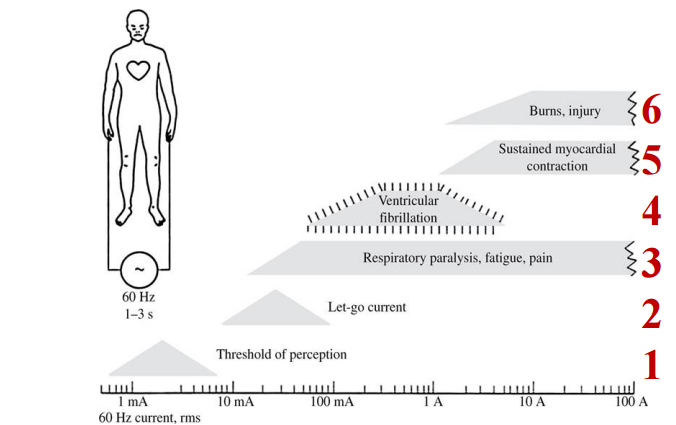
\includegraphics[scale=0.7]{figures/bProblemanalyse/Patientsikkerhed.png}
	\caption{Figuren viser effekten, som strømmen har på patienten ved forskellige strømstyrker og er inddelt i 6 stadier. Figurens gyldighed er forudsat, at personen har en vægt på 70 kg og er i kontakt med et elektronisk kredsløbet i 1-3 sekunder ved 60 Hz med begge hænder. \fxnote{Kilde er Webster2009, men den er ikke lagt ind i JabRef endnu (29/09)}}
	\label{Patientsikkerhed}
\end{figure}

På \figref{Patientsikkerhed} ses den effekt som elektrisk strøm kan have på patienten ved forskellige strømstyrker. Disse effekter kan opdels i seks forskellige stadier:

\begin{enumerate}
\item  I stadie 1 på \figref{Patientsikkerhed} findes den laveste strømstyrke på 0,5-10 mA. Ved dette stadie vil patienten føle en prikkende fornemmelse. Strømtætheden er stor nok til at aktivere nervesensorerne i huden, hvilket kan give en let opvarmning heraf. 

\item Ved stadie 2 på \figref{Patientsikkerhed} udsættes patienten for en elektrisk strøm mellem 10 mA og 100 mA. Dette er den maksimale strøm, hvor patienten kan afbryde kontakten frivilligt. Patienten vil opleve en kraftig påvirkning af muskler og nerver, hvilket resulterer i muskeltræthed og smerte, da musklerne skal lave ufrivillige kontraktioner.

\item I stadie 3 på \figref{Patientsikkerhed} er strømstyrken mellem 20 mA og 100 A og her kan patienten opleve åndedrætslammelser, smerter og muskeltræthed. Dette kan desuden resultere i kvælning, hvis strømmen ikke afbrydes. 

\item Ved stadie 4 på \figref{Patientsikkerhed}, som ligger mellem 75 mA og 4 A, kan patienten opleve ufrivillig kontraktion af hjertemuskulaturen, hvilket kan medføre ventrikelflimmer. 

\item I det 5. stadie på \figref{Patientsikkerhed} er strømstyrken mellem 1 A og 100 A. Her sker kontraktioner af hele hjertemuskulaturen. Dette kan resultere i hjertestop, da hjertet er konstant kontraheret og derfor ikke kan videregive elektriske signaler. 

\item Ved det 6. og sidste stadie på \figref{Patientsikkerhed} vil patienten opleve stærk strøm, som kan medføre alvorlige brandsår på huden. Ved store strømstyrker kan muskelkontraktionerne blive så kraftige, at musklen og knoglerne kan løsrive sig fra hinanden. Derudover vil hjernen og nervevæv miste alle funktioner, når store strømme løber gennem kroppen. Som det ses på \figref{Patientsikkerhed} kan flere af stadierne overlappe hinanden og foregå samtidig. \cite{Webster2009}
\end{enumerate}

\subsubsection{Makro- og mikrochok}

Der er forskellige muligheder for, hvordan den elektriske strøm løber igennem kroppen, hvilket bestemmer, hvor skadende strømmen er for patienten. De to forskellige muligheder er makro- og mikrochok. Makrochok sker, når strømmen løber igennem kroppen ved to punkter på hudens overflade og derved går kun en mindre del af strømmen igennem hjertet. Mikrochok sker, når det meste af strømmen løber igennem hjertet. Strømmen kommer fra et punkt på hudens overflade og forekommer hos patienter med elektriske ledere i hjertet f.eks. katetere. \cite{Webster2009}

Det er vigtigt at have fokus på patientsikkerhed, når der skal fremstilles medicinsk udstyr, som skal tilsluttes patienter. Dette kan gøres med en jordforbindelse i systemet eller ved at sørge for, der ikke er direkte kontakt mellem patienten og elnettet. Store mængder strøm kan have alvorlige konsekvenser for patientens heldbred.


\begingroup
	\raggedright
		\bibliographystyle{unsrtnat}
		\bibliography{VoresKilder}
\endgroup

%\begin{appendices}
%	\input{rapportAfsnit/yBilag/    .tex}
%\end{appendices}

\end{document}